\documentclass[11pt]{article}
\usepackage{tipa}
\usepackage{graphicx}
\usepackage{amsmath}
\usepackage{indentfirst}
\usepackage{cite}
\usepackage{listings}
\usepackage[makeroom]{cancel}
\usepackage{ulem}
\newcommand{\numpy}{{\tt numpy}}    % tt font for numpy
\topmargin -0.5in
\textheight 9in
\oddsidemargin -.25in
\evensidemargin -.25in
\textwidth 7in
\usepackage{xcolor}

\definecolor{codegreen}{rgb}{0,0.6,0}
\definecolor{codegray}{rgb}{0.5,0.5,0.5}
\definecolor{codepurple}{rgb}{0.58,0,0.82}
\definecolor{backcolour}{rgb}{0.95,0.95,0.92}

\lstdefinestyle{mystyle}{
    backgroundcolor=\color{backcolour},   
    commentstyle=\color{codegreen},
    keywordstyle=\color{magenta},
    numberstyle=\tiny\color{codegray},
    stringstyle=\color{codepurple},
    basicstyle=\ttfamily\footnotesize,
    breakatwhitespace=false,         
    breaklines=true,                 
    captionpos=b,                    
    keepspaces=true,                 
    numbers=left,                    
    numbersep=5pt,                  
    showspaces=false,                
    showstringspaces=false,
    showtabs=false,                  
    tabsize=2
}
\lstset{style=mystyle}


\begin{document}
\author{%
  Xifan Yu, \hspace{0.9in} Yiyang Ou, \hspace{0.9in} Zixuan Alex Zhao\\
 \texttt{xifan@uchicago.edu, yiyangou@uchicago.edu, zhaozixuan@uchicago.edu}}
\title{Raft Made Live: A Simple Python Implementation }
\maketitle


\section{Introduction}

Consensus algorithms are essential to building a consistent distributed system. Paxos \cite{Paxos} was an early consensus algorithm developed to achieve data consistency. However, Paxos is also considered as a hard-to-understand protocol, and since its publication, scientists have been searching for consensus algorithms that are more intuitive and are more suitable for building practical distributed system. Raft \cite{Raft} was among one of them. It is a protocol equivalent to (multi-)Paxos, and it is as efficient as Paxos. Its different structure from Paxos makes Raft more understandable than Paxos, and also provides a better foundation for building practical systems. Raft separates the key elements of an consensus algorithm, such as leader election, log replication, and safety, and this greatly enhances its understandability.

Section 2 covers an overview of the Raft algorithm and consensus algorithms in general. Section 3 describes the implementation details about our projects and section 4 shows the types of faults that our program can tolerate and how they are tolerated. Section 5 provides a detailed description of our testing toolkits and testcases. Section 6 discusses various issues, challenges, and lessons in this project. Finally, section 7 gives a summary of this project.

\section{Raft Overview}

\subsection{Properties of Consensus Algorithms}

Consensus algorithms for practical systems typically have the following properties [2]:
\begin{itemize}
    \item They ensure safety (never returning an incorrect result) under all non-Byzantine conditions, including network delays, partitions, and packet loss, duplication, and reordering.
    \item They are fully functional (available) as long as any majority of the servers are operational and can communicate with each other and with clients. Thus, a typical cluster of five servers can tolerate the failure of any two servers. Servers are assumed to fail by stopping; they may later recover from state on stable storage and rejoin the cluster.
    \item They do not depend on timing to ensure the consistency of the logs: faulty clocks and extreme message delays can, at worst, cause availability problems.
    \item In the common case, a command can complete as soon as a majority of the cluster has responded to a single round of remote procedure calls; a minority of slow servers need not impact overall system performance.
\end{itemize}

Raft is a protocol that implements a consensus algorithm, which satisfies the above properties.

\subsection{The Raft Consensus Algorithm}

A Raft cluster contains several servers: five is a typical number, which allows the distributed system to tolerate two failures. In Raft algorithm, each server is in one of three states: \textit{leader}, \textit{follower}, or \textit{candidate} (Figure $1$). In normal operation, there is exactly one leader, and all other servers act as followers. Followers only respond to requests from other servers. If a follower cannot identify the presence of a leader for a while, it will transit to candidate state, and initiate a new election through \texttt{RequestVote} RPC. If the candidate receives votes from a majority of the full cluster, then it becomes a new leader and periodically sends out heartbeats to establish its authority.

Raft implements consensus by first electing a distinguished leader, and then asking the leader to manage all client requests and ensure consistency across the servers. All other servers that receive requests will redirect the requests to the leader they are following. The leader is responsible for accepting log entries from clients, replicating these entries on other servers, and telling the servers when to safely apply the log entries.

Following the leader based approach, Raft decomposes the consensus problem into three relatively independent subproblems:
\begin{itemize}
    \item \textbf{Leader election}: a new leader must be elected when there is no current leader.
    \item \textbf{Log replication}: the leader must accept log entries from clients and replicate them across the cluster, enforcing log consistency.
    \item \textbf{Safety}: if any server has applied a particular log entry to its state machine, then no other server may apply a different command for the same log index.
\end{itemize}

\begin{figure}[h]
  \centering
    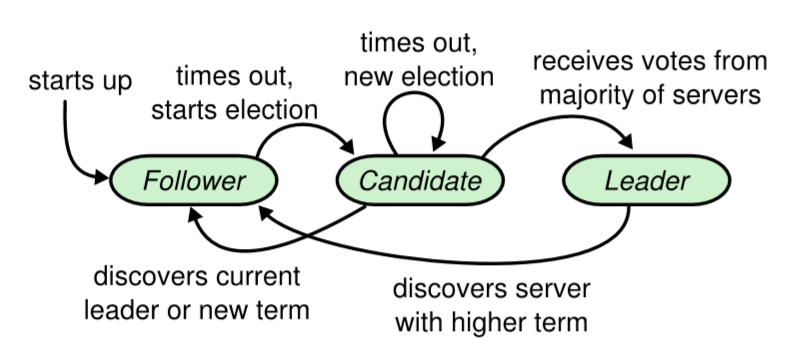
\includegraphics[scale=0.4]{transitions.PNG}
    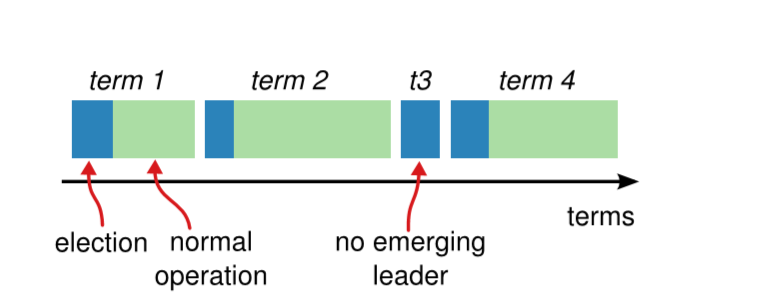
\includegraphics[scale=0.4]{term.PNG}
  \caption{Server states and terms illustration \cite{Raft}}
  \label{fig:speech_production}
\end{figure}


\subsection{Leader Election}

When a leader is present in the system, it periodically sends heartbeats to all followers in order to maintain their authority. If a follower does not hear from a leader over a period of time called the election timeout, then it transits to candidate state and initiates a new election.

The election proceeds in the following way:
\begin{enumerate}
    \item The follower increments its current term, and transits to candidate state.
    \item It votes for itself, and issues \texttt{RequestVote} RPCs.
    \item The candidate remains in current state until one of the following happens:
    \begin{itemize}
        \item It wins the election by receiving votes from a majority of servers. In this case, the candidate transits to leader state.
        \item Another server establishes itself as leader, and has term at least at large as the candidate's current term. In this case, the candidate reverts to follower state.
        \item Neither does it receive votes from a majority of servers, nor has it identified a new leader in the cluster. In this case, the candidate restarts an election.
    \end{itemize}
\end{enumerate}

The third case above happens when votes are split evenly across the cluster. Raft uses randomized election timeouts to ensure that split votes are rare and that they are resolved quickly. Election timeouts for each server are chosen randomly from an interval. [2] shows that this approach elects a leader rapidly after split votes happened.




\subsection{Log Replication}
Once leaders are elected, leaders maintain the log by appending the incoming commands from the clients and issues \texttt{AppendEntries} RPC so that other servers could replicate the entry. The entries are applied to the state machine once it is safely replicated.

A log entry is committed once the leader has replicated it on a majority of the servers. 
If followers crash or packets are lost, leaders would retry \texttt{AppendEntries} RPC indefinitely.

The leaders keep track of the highest index it knows to be committed, and it includes the index in future \texttt{AppendEntries} RPCs so that the other servers eventually would find out. Once the followers learn that a log entry is committed, it applies the entry to its local state machine in log order as well. The Log Matching Property is constituted by the following two rules: if entries in different logs have the same index and term, 
\begin{itemize}
    \item They store the same command
    \item The logs are identical in all preceding entries. 
\end{itemize}

These two requirements would ensure that when \texttt{AppendEntries} returns successfully, the leader knows that the follower’s log is identical to its own log up through the new entries. 

In the case of leader failures, Raft handles inconsistencies by forcing the followers’ logs to duplicate its own. This means that the conflicting entries in the follower logs will be overwritten with entries from the leader’s log. Specifically, the leader keeps track of \texttt{nextIndex} for each follower, which is the index of the next log entry the leader will send to that follower. The leader then decrements the \texttt{nextIndex} value until it reaches a point where the follower and leader logs match. \texttt{AppendEntries} then succeed and removes conflicting entries in the follower’s log. Note that this also follows the Leader Append-Only Property as logs only flow from the leaders to the followers. 
\subsection{Safety}
In the section 5.4 \cite{Raft}, the authors talked about additional restrictions of the Raft algorithms, including which servers maybe selected as leaders and which logs could be committed from previous terms. They also gave a proof sketch for Leader Completeness Theorem.

Raft restricts the election process by preventing candidates winning the election unless its log contains all committed entries. During voting, candidate must contact a majority of the clusters to be elected and if the candidate’s log is at least up-to-date as any other log in that majority, then it will hold all the committed entries. 

If leader crashes before committing an entry, future leaders will attempt to replicate the entry. However, terms from previous terms are committed not by counting replicas, but instead replying on the Log Matching Property - all prior entries are committed indirectly. Raft does this additional requirement in commitment rules because log entries retain their original term numbers when leaders replicate entries from previous terms. 

\section{Implementation}

In this section, we briefly discuss our implementation details. Our implementation is built on \texttt{chistributed} and \texttt{pyzmq}. The core part of our code is built on the \texttt{Node} class provided within \texttt{node.py}, which provides handlers for various message types, including but not limited to:
\begin{itemize}
    \item \texttt{appendEntries / appendEntriesResponse}
    \item \texttt{requestVote / requestVoteResponse}
    \item \texttt{redirectSet / redirectGet / redirectSetResponse / redirectGetResponse}
    \item \texttt{set / get}
    \item \texttt{hello}
\end{itemize}

In this section, we will talk more specifically about their functionalities and how they work together in the context of Raft. 
\subsection{General}

\subsubsection{Leader Detection}

Following the leader based approach, we need to design a method for each server to check for heartbeats sent from the leader. We achieve this by starting a new thread at the startup of each node that runs a function called \texttt{leader\_detection\_loop()}. This loop keeps running in the background till the node shuts down at the end of the program.

In this loop, after an election timeout the server checks for heartbeats received if it is in follower state. If a heartbeat was detected, the follower recognizes the sender of that heartbeat as the leader, and will redirect all get and set operations to the leader. If a heartbeat was not detected over the period, the follower assumes that there is no leader present in the cluster, and calls RequestVote RPCs as a candidate to initiate a new election.


\subsubsection{Heartbeat Propagation}

The leader needs to periodically send out heartbeats to maintain its authority over its term. We achieve this by starting a new thread when the server has become leader, running a function called \texttt{heart\_beat\_loop()}.

In this loop, as long as the server is still in leader state, it sends out heartbeats (AppendEntry RPCs without log entries) to all other servers in the cluster. When it exists leader state, the thread running this loop is joined.

\subsubsection{Redirection}
According to Raft paper, the leader handles all the client requests. When client contacts a follower, the follower would redirect it to the leader. This is implemented not only by including a leader id field in the \texttt{AppendEntries} responses but also a custom message type for \texttt{set} and \texttt{get} operations. When follower nodes received \texttt{set} and \texttt{get} operations,
it sends a redirect message to the current term leader. It sets up a timer concurrently and will timeout if leader does not respond timely. This could happen when the leader fails, the follower fails, or they are in different partitions. In these cases, error message will be returned saying leader timeout. It might also be possible the follower doesn't have a current term leader if a election is ongoing. In this case, error message is also returned saying there is no leader.

\subsubsection{Round Trip}
According to Raft paper in section 8, to make sure linearizable reads don't return stale data, the leader must check if it's still a leader before processing \texttt{get} request. In our implementation, the leader achieves this by running a "round trip" before processing \texttt{get} request. In a round trip, the leader sends a message to all other nodes and wait for response. A follower node receiving the message will respond only if the leader is still its leader. Once leader receives more than majority of response, it will process the \texttt{get} request. On the other hand, if leader doesn't receive enough response in given time, it will timeout and respond "leader stale" error message to \texttt{get} request and also revert to follower state. This mechanism is important to ensure we don't read stale data when partitioning happens, which will be described in section 4.2.

\subsection{Leader Election}

In Raft algorithm, the leader election process starts when a follower has not received a heartbeat in the function \texttt{check\_heart\_beat()} during the execution of \texttt{leader\_detection\_loop()} over a period time. Then, the follower transits to candidate state and calls the function \texttt{request\_vote()}.

In the function \texttt{request\_vote()}, the candidate will enter a loop that keeps restarting a new election until the function \texttt{check\_vote()} indicates the election result has been resolved, i.e., either the candidate has been elected as leader, or the candidate has reverted back to follower state because another leader appeared.

When a new election starts, the candidate first increments its term by $1$, and sets the vote count \texttt{self.votes} to $1$ since it votes for itself. Then, the candidate sends out messages of the type \texttt{requestVote} to all other servers in the cluster, and calls the function \texttt{check\_vote()} after an election timeout to determine if it needs to exit the loop (when the election has been resolved), or stay in the loop to restart a new election (when a split votes happened).

On receiver side, when a server receives \texttt{requestVote} message from a candidate, it checks the following conditions before responding to the request. If the log entries of the candidate (sender of the \texttt{requestVote} message) is at least as up-to-date as the receiver's log, and either the receiver has not voted in its current term or the receiver has voted for this same candidate before, then the receiver will grant its vote to the candidate by sending back a message of the type \texttt{requestVoteResponse} with the \texttt{vote} field in the message set to \texttt{True}. Otherwise, the receiver sends back a message of the type \texttt{requestVoteResponse} with the \texttt{vote} field in the message set to \texttt{False}. The \texttt{requestVoteResponse} message also sends back the term of candidate running the election, in order for the candidate (receiver of \texttt{requestVoteResponse} message) to distinguish between responses to previous elections and current election it is running.

On candidate side, when a candidate receives \texttt{requestVoteResponse} message, it first checks if the message is responding to its current election by comparing its current term with the \texttt{term} field in the response message. If the message is responding to its current election, it will check for the \texttt{vote} field in the response message, and increment \texttt{self.votes} by $1$ if the \texttt{vote} field is set to \texttt{True}. If the candidate gathers votes from a majority of the cluster after receiving this message, it will transit to leader state and start a new thread running the function \texttt{heart\_beat\_loop()} that sends out heartbeats to other servers in the cluster to establish its authority.

A candidate might also receive an \texttt{appendEntries} message during its election. In this case, if the \texttt{term} of the sender of this message (the leader) is at least as large as the candidate's, the candidate quits its election and reverts back to follower state. Otherwise, the candidate stays in its election.



\subsection{Log Replication}

In section 3.1, we talked about the implementation of redirect mechanism. When followers received get and set messages, they are handled by the \texttt{getFollowerHander} and \texttt{setFollowerHanlder}, where timers are initiated and redirect messages are sent to the broker. When leaders received set and get messages, they are handled by \texttt{setOperation} and \texttt{getOperation}. 

As mentioned in section 3.1.4, the leader first checks if it's still the leader by calling \texttt{roundTrip} before executing the \texttt{getOperation}. \texttt{getOperation}, which implements the actual reading of data store, is straightforward, just by checking if its datastore contains the requested key. In \texttt{setOperation}, we  wait until hearing back from a majority of the peers so that we can append the entries to the log. This propagation of message is implemented by checking the \texttt{AppendEntriesReponse} message and \texttt{append\_entries\_has\_log} function. We also used the optimization mentioned in section 5.3 \cite{Raft} where a match index array is used to apply chunk of logs at the same time. 

From the follower’s side, after checking the leader’s current term and \texttt{preLogIndex} is matched, we apply the entries sent from the leaders and update commit index. The commit index is updated to the minimum of length of log and the \texttt{leaderCommit} field in the message. Then we respond to the leader an \texttt{appendEntriesResponse} message and set the flag as \texttt{True}. If either of the two criterion failed, we returned with flag as \texttt{False}. From the leaders’s side, if the append flag is set as \texttt{True}, we used the \texttt{update\_commit} function to update commit index for the leaders. If a majority of the match indexes are larger than the current log index, we apply the current log block. 

When applying the log entries, the node stores the key value pair in the \texttt{store}, which is implemented dictionary simulating a stores.

\section{Fault Tolerance}

In this section, we list the errors our program can tolerate, and briefly discuss how each error is tolerated. There are two errors that our program can handle:
\begin{itemize}
    \item Fail-stop: this is an abstraction of the crash error. It happens when a server no longer responds to the messages from other servers in cluster.
    \item Network-partition: this happens when the cluster is split into several components. In this partition, communication between different components is blocked, and servers can only communicate to servers in the same component.
\end{itemize}

\subsection{Fail-Stop}

When the leader failed, other servers in the cluster no longer receives heartbeats from the leader, and assumes that no leader is present. Therefore, some of them will transit to candidate state and start an election. As long as the number of functional servers in the cluster is more than half of the total number of servers in the cluster, the remaining servers will be able to elect a new leader and proceed in normal operation.

If a follower fails, since in Raft, log replication only flow from the leader to follower, this would not cause a problem if we are only dealing with fail-stop problems. If the log exists on a majority of the nodes, it would be applied in a later term according to the election restriction in section 5.3 \cite{Raft}. If it does not exist on a majority of the nodes, it could be overwritten in a later section.  The new leader will automatically simulates as it has received a dummy set request, which triggers a round of log replication to its quorum, which will commit entries that are the uncommitted but already existing on majority of nodes. Therefore, our code should be resilient to fail-stop errors during log replications. 


\subsection{Network Partition}

When the network is partitioned into components, exactly one of the following happens:
\begin{itemize}
    \item In the partition, there is one component that contains a majority of servers in the original cluster, and the remaining components do not contain a majority of servers.
    \item No component in this partition contains a majority of servers in the original cluster.
\end{itemize}

In either case, the components in the partition that do not contain the leader in the original cluster will not be able to reach the leader. The servers in those components will not detect heartbeats, and transit to candidate state to initiate new elections. If an election takes place in a component that does not contain a majority of servers, the election will never resolve. If an election takes place in a component that contains a majority of servers, the election will eventually resolve. If the old leader is in a partition without majority of nodes, it is not able to commit any logs because there are not enough servers in its component and if client calls \texttt{get} on this leader, it will not get enough response from round trip which will cause it to timeout and return to a follower. This step of round trip is necessary because if a new leader is already elected in the larger partition, but a client chooses to read from the old leader, then it will read stale data.

Therefore, in the former case, the component that contains a majority of servers will be fully functional, and other components either do not have a leader, or have a leader will respond error to \texttt{get} and \texttt{set}. In the latter case, no component will be able to process any requests, and all requests will eventually timeout and errors will be returned.



\section{Testcase Analysis}

We include 5 test scripts to illustrate functionalities discussed before. {\bf{test1}} {\bf{test2} \bf{test3}} have configuration of 5 nodes, {\bf test4} has 4 nodes and {\bf test5} has 7 nodes. We explain the purpose of each test and how our system behaves in each test. We call the nodes as \texttt{node-1},\texttt{node-2}... And at the beginning stage of each test, we will start each node and use \texttt{wait -t} to wait for the first leader to be elected. 

We provide the testing script that runs all following test cases: \texttt{run\_test.sh}. Scripts would setup the corresponding configuration files and input the \texttt{chistributed} commands under \texttt{scripts/chi/}. The output file is stored under \texttt{scripts/output}. And our submission already contains the output we ran for {\bf{test1}}, {\bf{test2} \bf{test3}, test4, test5}. We also provided script that runs only 1 test. See more about testing at the \texttt{README.md} file under \texttt{script/}. 

\begin{lstlisting}[language=bash]
for test_case in $(seq 1 $tot_test); do
    cp ./scripts/conf/test$test_case.conf ./chistributed.conf
    echo "Running test case $test_case"
    test_file=./scripts/chi/test$test_case.chi
    output_file=./scripts/output/test_output$test_case.txt
    echo "stored at: "$output_file
    timeout 40 chistributed --pub-port 23310 --router-port 23311 < $test_file > $output_file
done
\end{lstlisting}

\subsection{Set and Get}

{\bf test1} shows \texttt{get}  and \texttt{set} work properly when there are no node failures. Specifically, we \texttt{set} different key-value pairs on \texttt{node-1},\texttt{node-2},...,\texttt{node-5}. Suppose \texttt{node-1} is the leader. A follower node, such as \texttt{node-2}, will redirect its received \texttt{set} request (say key-value pair (B,2)) to leader, and the leader replicates the key-value pair and applies it to its store. After this, because of redirection and replication, we can successfully call \texttt{get} on \texttt{node-3}  asking for the value of key \texttt{B} even though we didn't explicitly \texttt{set} (B,2) on  \texttt{node-3}.


\subsection{Fail Gracefully}
{\bf test2} shows \texttt{get} and \texttt{set} return correct error message when called on a failed node: \texttt{node-1}. One caveat is since Raft uses randomized election timeout, this failed node can either be a leader or a follower. Hence, the error message might vary in different runs: if \texttt{node-1} is a leader, \texttt{set} will timeout after leader realizing it can't replicate the log on majority of nodes, and \texttt{get} will fail saying leader is stale because round trip can't get responses; on the other hand, if \texttt{node-1} is a follower, \texttt{set} and \texttt{get} will both say leader timeout because its redirect message can't be received by leader; last case is if \texttt{node-1} fails and starts a new election, but it can't resolve election because it can't receive votes from others. Then, \texttt{node-1} will say "no leader" error to both \texttt{set} and \texttt{get}, since Raft system can serve client only when a leader is present. 


\subsection{Fail-Stop}
{\bf test3} shows the system is resilient to single node failure: \texttt{node-1}, whether it's a leader or a follower, if majority of nodes are still alive. After \texttt{node-1} fails, if it's follower fails, the system is not affected. If it's leader fails, one of \texttt{node-2},\texttt{node-3},\texttt{node-4},\texttt{node-5} will cause election timeout because they can't receive heart beats from \texttt{node-1}. Then a new leader will be elected, say \texttt{node-2}, and it starts servicing requests with a new leader. It's possible there are log entries replicated on majority of machine and committed on the \texttt{node-1}, but not yet committed on the \texttt{node-2}. \texttt{node-2} will automatically simulates as it has received a dummy \textt{set} request, which triggers a round of log replication to its quorum, which will commit the uncommitted entries. After this, because majority of nodes are still alive, the system behaves the same way as in {\bf test1} in the eye of client, i.e. \texttt{get} and \texttt{set} should succeed. 


\subsection{Network Partition}
{\bf test4} and {\bf test5} both test network partition. In {\bf test4}, we divide 4 nodes into two partitions each with 2 nodes, so neither partition contains a majority of node. As a result \texttt{set} and \texttt{get} on the partition with a leader will timeout after leader realizing it can't replicate the log on majority of nodes, and will say the stale leader since round trip will fail. On the partition without a leader, new leader election can't succeed because the partition doesn't have majority of nodes, so \texttt{set} and \texttt{get} will either say leader timeout (if they haven't started reelection and are in follower state) or no leader exists (if they enter reelection and become candidates). In {\bf test5}, we divide 7 nodes into two partitions one with 2 nodes and one with 5 nodes (\texttt{node-3},..,\texttt{node-7}), so 5-node partition has majority of nodes. Then 5-node partition will reelect a new leader if old leader is in (\texttt{node-1},\texttt{node-2}) or is not affected if old leader is already in (\texttt{node-3},..,\texttt{node-7}). Then, due to similar reasoning in {\bf 5.3}, the new leader will simulate a dummy \texttt{set} to commit any previously uncommitted but replicated logs. Then, 5-node partition will service requests with the new leader and \texttt{set} and \texttt{get} will both succeed.

\section{More Discussion}
\subsection{Limitations}
There are some limitations of script testing due to the randomness nature of Raft election and reelection.
One is we do not know who becomes a leader. If one wants to test leader failure specifically, one can run \texttt{chistributed --show-node-output} in terminal mode, which allows one to see who becomes the leader. Then one could fail that node specifically to test leader failure.

Another limitation is we have to add \texttt{wait -t} after failing the leader or at start up to allow enough time for a new leader to be elected, before calling \texttt{get} and \texttt{set} command. Otherwise, \texttt{get} and \texttt{set} will generate "no leader" error, since election hasn't been completed. 

\subsection{Observations}

\begin{figure}[h]
  \centering
  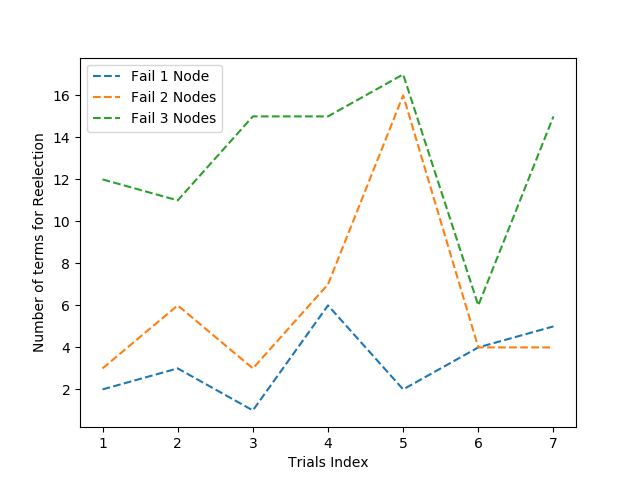
\includegraphics[width=10cm, height=8cm]{Num_terms_reelection.png}
  \caption{Number of terms needed for reelection}
  \label{fig:speech_production}
\end{figure}


One more interesting observation about Raft algorithm is that the number of terms (time) needed for leader reelection varies according to the number of nodes alive. For example, we performed a experiment with $8$ nodes. Each time, we start up all the nodes. After the leader has been elected, we fail $k = 1,2,3$ nodes including the leader, and we keep track of the number of terms that passed before a new leader is elected. Figure $2$ shows that

\begin{itemize}
    \item When $1$ node is failed, there are $7$ nodes alive. In this case, a candidate needs to gather $5$ votes from the $7$ nodes alive to become the new leader. The blue line in the figure shows that the remaining nodes reelect a new leader pretty rapidly, using only $3$ or $4$ terms.
    \item When $2$ nodes are failed, there are $6$ nodes alive. In this case, a candidate needs to gather $5$ votes from the $6$ nodes alive to become the new leader. The orange line in the figure shows that they need a little bit more time for reelection of the new leader. The number of terms needed is around $6$ or $7$.
    \item When $3$ nodes are failed, there are only $5$ nodes alive, which is exactly the number of nodes that constitutes a majority of a cluster of $8$ nodes. In this case, a candidate needs to gather all votes from the $5$ nodes alive to become the new leader. The green line in the figure shows that they took significantly longer time in order to reelect a new leader: the average number of terms needed is around $13$.
\end{itemize}

\subsection{Challenges and Lessons}
During implementation, we encountered many times KeyError from the pyzmq library and we realized that it was due to concurrency issues at the startup of nodes. For example, pyzmq might send \texttt{get} messages to the nodes before it is initialized. Therefore, when pyzmq queried the name of the node, it is set to \textt{None}, which caused the KeyError mentioned above. We solved this by only allowing \texttt{Hello} messages to be delivered to nodes when nodes are not connected. 

Another thing was we were not very familiar Python threading library. For example, we forgot to wait for threads to finish when shutting down the node, which caused many strange error messages and missing of expected output. We got more experienced with how to handle threads throughout the project and become able to efficiently use Timer to implement request timeout, etc.

Lastly, since there are not enough documentations on the \texttt{chistributed} commands, we had some trouble using the infrastructure. It seems that \texttt{quit} command is not working from the \texttt{chistributed} framework and we have communicated with other groups and TA: we decided to use a GNU command \texttt{timeout} to terminate the bash script if it fails to stop. We also realized the importance of automated testing scripts: it saved a lot trouble when we are trying to conduct experiments for multiple times (provided under \textt{Impl}). Another issue is that we cannot add custom fields to the \texttt{set} and \texttt{get} messages because they are instantiated from the \texttt{cmd} and \texttt{interpreter} module. To circumvent this, we used a custom message field \texttt{redirectGet} and \texttt{redirectSet} to redirect the messages to the leaders.


\section{Conclusion}

In this project, we implemented a simplified version of the Raft algorithm that is resilient to fail-stop errors and network partitions. The Raft algorithm is easily understandable in that it separates the key elements of consensus algorithms, such as leader election, log replication, and safety, and it enforces a stronger degree of coherency to reduce the number of states that must be considered. Our implementation of the \texttt{appendEntries} and \texttt{update\_commit} logic follows directly from the Raft paper \cite{Raft} and ensures that reelections would occur and system would go back to normal when leader fails. We also look into the relation between the numbers of failed nodes and the length of reelection process in section 5. 

\begin{thebibliography}{9}
\bibitem{Paxos} 
Lamport, L. 
\textit{Paxos made simple}. 
ACM Sigact News 32, no. 4 (2001): 18-25


\bibitem{Raft}
Ongaro, D., and Ousterhout, J. \textit{In search of an understandable consensus algorithm}. In 2014 \{USENIX\} Annual Technical Conference (\{USENIX\}\{ATC\} 14), pp. 305-319. 2014.


\end{thebibliography}


\end{document}
